\documentclass[12pt,a4paper]{article}

% Margins.
\setlength{\oddsidemargin}{0in}
\setlength{\evensidemargin}{0in}
\setlength{\headheight}{12pt}
\setlength{\headsep}{42pt}
\setlength{\topmargin}{-54pt}
\setlength{\textwidth}{6.5in}
\setlength{\textheight}{10in}
\pagestyle{plain}

\usepackage{amsmath}
\usepackage{float}
\usepackage{graphicx}
\usepackage[hyphens]{url}
\usepackage[hidelinks]{hyperref}	% Clickable links to figures, references and urls.
\usepackage{lastpage}
\usepackage{ulem}

% Drawing.
\usepackage{pgf}
\usepackage{tikz}

% Listings for formatting code.
\usepackage{listings}
\usepackage{textcomp}
% General options.
\lstset{breaklines=true, basicstyle=\footnotesize\ttfamily, tabsize=4, numbers=none, stepnumber=1, frame=single, showstringspaces=false, upquote=true}
% C++ specific high-lighting. Comments are 50/50 shades of green/black and strings coloured with 60/40 red/black mixture.
\lstset{language=[ISO]C++, commentstyle=\color{green!50!black}, keywordstyle=\color{blue}, stringstyle=\color{red!60!black}}

% Marks of each question.
\def\QOne{2}
\def\Qtwo{2}
\def\Qthree{2}
\def\Qfour{2}
\def\Qfive{2}
\def\TotalMarks{10}

\begin{document}
\begin{minipage}{0.55\textwidth}
{\LARGE \textbf{Programming for\\ Engineers I -- Lab}}\\[0.15cm]
{\normalsize \textbf{Spring 2013 Semester}}\\
{\Large {Final Exam (Written)}}\\
{\normalsize \textbf{Tuesday, May 28, 2013}}\\[0.30cm]
{\Large \textbf{Total Time: 30 minutes}}\\[0.15cm]
{\Large \textbf{Total Marks: 10}}\\
\textbf{Course Instructor:}\\
Attique Dawood\\
\end{minipage}
\begin{minipage}{0.4\textwidth}
\textbf{Serial} \hrulefill \\[0.25cm]
\textbf{Name} \hrulefill\\[0.25cm]
\textbf{Section} \rule{1cm}{0.2mm} \textbf{Roll No:} \hrulefill\\[0.25cm]
\textbf{Signature:} \hrulefill\\[0.25cm]
\rule{6.6cm}{0.2mm}\\
\textbf{Signature of Invigilator}\\[0.25cm]
\end{minipage}
\begin{table}[H]
\begin{center}
\vspace{0.3cm}
	{\Large \begin{tabular}{|l|c|c|c|c|c|c|}
	\hline
		\rule{0pt}{2.6ex} Question & \textbf{1} & \textbf{2} & \textbf{3} & \textbf{4} & \textbf{5} & \textbf{Total}\\
		\hline
		Total Marks \rule{0pt}{2.6ex} & \QOne & \Qtwo & \Qthree & \Qfour & \Qfive & \TotalMarks\\
		\hline
		Marks Obtained & & & & & & \\
	\hline
	\end{tabular}}
\end{center}
\end{table}
\noindent \textbf{You are advised to READ these notes:}
\begin{enumerate}
\item \textbf{Attempt on the Question Paper. \underline{NO EXTRA SHEET} will be provided/accepted. No
additional sheet will be provided for rough work. Use the back of the page where
provided space is not sufficient.}
\item After asked to commence the exam, please verify that you have \textbf{\pageref{LastPage} different
printed pages} including this title page.
\item There are 5 questions. Attempt all of them. It is advisable to go through the paper once
before starting with the first question.
\item Exam is closed books, closed notes. Please see that the area in your threshold is clean.
You will be charged for any material which can be classified as \textbf{`helping in the paper'}
found near you.
\item \textbf{Calculator sharing is strictly prohibited.}
\item Students who attempt the paper with lead pencils lose the right to get them rechecked.
\item \textbf{The invigilator present is not supposed to answer any questions. No one may come
to your room for corrections and you are not supposed to request to call anyone.
Make assumptions wherever required and clearly mark them.}
\end{enumerate}
\newpage
\noindent\textbf{Question 1: What is the keyword for,\hfill \QOne~marks}\\
\begin{enumerate}
\item[a.] Dynamic allocation of memory.
\begin{figure}[H]
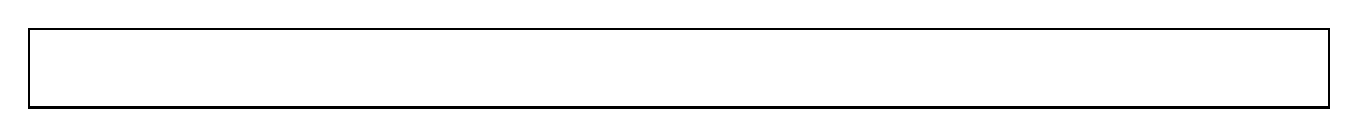
\begin{tikzpicture}
	\draw[thick] (0cm,0cm) rectangle (\textwidth, 1cm);
\end{tikzpicture}
\end{figure}
\item[a.] De--allocation of memory.
\begin{figure}[H]
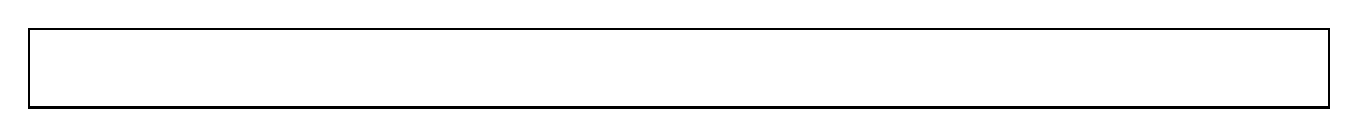
\begin{tikzpicture}
	\draw[thick] (0cm,0cm) rectangle (\textwidth, 1cm);
\end{tikzpicture}
\end{figure}
\end{enumerate}
\noindent\textbf{Question 2: How much space is taken by \texttt{float x $=$ -2.74393;}\hfill \Qtwo~marks}\\
\begin{enumerate}
\item[a.] If stored in a text file.
\begin{figure}[H]
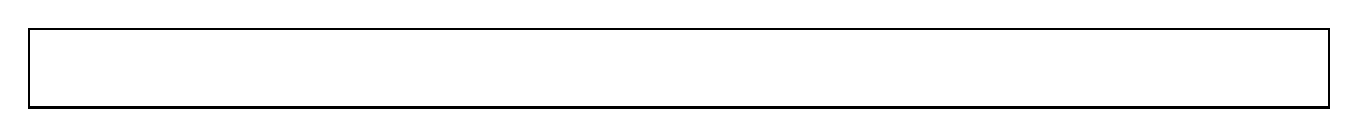
\begin{tikzpicture}
	\draw[thick] (0cm,0cm) rectangle (\textwidth, 1cm);
\end{tikzpicture}
\end{figure}
\item[a.] If stored in binary file.
\begin{figure}[H]
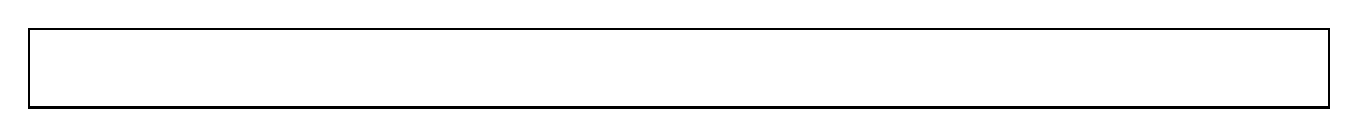
\begin{tikzpicture}
	\draw[thick] (0cm,0cm) rectangle (\textwidth, 1cm);
\end{tikzpicture}
\end{figure}
\end{enumerate}
\noindent\textbf{Question 3: Convert 129 to 8 bit unsigned binary notation.\hfill \Qthree~marks}\\
\begin{figure}[H]
\begin{tikzpicture}
	\draw[thick] (0cm,0cm) rectangle (\textwidth, 3cm);
\end{tikzpicture}
\end{figure}
\noindent\textbf{Question 4: Convert -1 to 4 bit signed binary notation.\hfill \Qfour~marks}\\
\begin{figure}[H]
\begin{tikzpicture}
	\draw[thick] (0cm,0cm) rectangle (\textwidth, 3cm);
\end{tikzpicture}
\end{figure}
\noindent\textbf{Question 5: In 32 bit float notation how many bits are reserved for\\ mantissa?\hfill \Qfive~marks}\\
\begin{figure}[H]
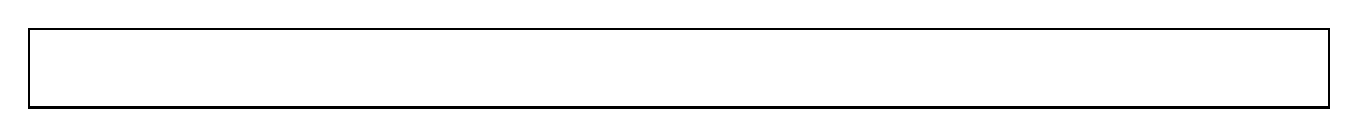
\begin{tikzpicture}
	\draw[thick] (0cm,0cm) rectangle (\textwidth, 1cm);
\end{tikzpicture}
\end{figure}

\end{document}